\documentclass[paper=letter,fontsize=11pt]{scrartcl} % KOMA-article class
							
\usepackage[english]{babel}
\usepackage[utf8x]{inputenc}
\usepackage[protrusion=true,expansion=true]{microtype}
\usepackage{amsmath,amsfonts,amsthm}     % Math packages
\usepackage{graphicx}                    % Enable pdflatex
\usepackage[svgnames]{xcolor}            % Colors by their 'svgnames'
\usepackage{geometry}
	%\textheight=700px                    % Saving trees ;-)
%\usepackage{url}
\usepackage[colorlinks=true,
linkcolor=blue,
urlcolor=blue]{hyperref}
\usepackage{float}
\usepackage{etaremune}
\usepackage{wrapfig}

\usepackage{attachfile}

\frenchspacing              % Better looking spacings after periods
\pagestyle{empty}           % No pagenumbers/headers/footers

%\addtolength{\voffset}{-40pt}
%\addtolength{\textheight}{20pt}

\setlength\topmargin{0pt}
\addtolength\topmargin{-\headheight}
\addtolength\topmargin{-\headsep}
\setlength\oddsidemargin{0pt}
\setlength\textwidth{\paperwidth}
\addtolength\textwidth{-2in}
\setlength\textheight{\paperheight}
%\addtolength\textheight{-3in}
\addtolength\textheight{-2in}
\usepackage{layout}

%%% Custom sectioning}{sectsty package)
%%% ------------------------------------------------------------
\usepackage{sectsty}

\sectionfont{%			            % Change font of \section command
	\usefont{OT1}{phv}{b}{n}%		% bch-b-n: CharterBT-Bold font
	\sectionrule{0pt}{0pt}{-5pt}{1pt}}

%%% Macros
%%% ------------------------------------------------------------
\newlength{\spacebox}
\settowidth{\spacebox}{8888888888}			% Box to align text
\newcommand{\sepspace}{\vspace*{1em}}		% Vertical space macro

\newcommand{\MyName}[1]{ % Name
		\Huge \usefont{OT1}{phv}{b}{n} \hfill #1
		\par \normalsize \normalfont}
		
\newcommand{\MySlogan}[1]{ % Slogan}{optional)
		\large \usefont{OT1}{phv}{m}{n}\hfill \textit{#1}
		\par \normalsize \normalfont}

\newcommand{\NewPart}[2]{\section*{\uppercase{#1} \small \normalfont #2}}

\newcommand{\NewParttwo}[1]{
		\noindent \huge \textbf{#1}
        \normalsize \par}



\newcommand{\PersonalEntry}[2]{\small
		\noindent\hangindent=2em\hangafter=0 % Indentation
		\parbox{\spacebox}{        % Box to align text
		\textit{#1}}		       % Entry name}{birth, address, etc.)
		\small\hspace{1.5em} #2 \par}    % Entry value

\newcommand{\SkillsEntry}[2]{      % Same as \PersonalEntry
		\noindent\hangindent=2em\hangafter=0 % Indentation
		\parbox{\spacebox}{        % Box to align text
		\textit{#1}}			   % Entry name}{birth, address, etc.)
		\hspace{1.5em} #2 \par}    % Entry value	
		
\newcommand{\EducationEntry}[4]{
		\noindent \textbf{#1} \hfill      % Study
		\colorbox{White}{%
			\parbox{6em}{%
			\hfill\color{Black}#2}} \par  % Duration
		\noindent \textit{#3} \par        % School
		\noindent\hangindent=2em\hangafter=0 \small #4 % Description
		\normalsize \par}

\newcommand{\WorkEntry}[5]{
		\noindent \textbf{#1}
        \noindent \small \textit{#2}
        \hfill      % Study
        \colorbox{White}{%
			\parbox{6em}{%
			\hfill\color{Black}#3}} \par  % Duration
		\noindent \textit{#4} \par        % School
		\noindent\hangindent=2em\hangafter=0 \small #5 % Description
		\normalsize \par}

\newcommand{\Language}[2]{
		\noindent \textbf{#1}
        \noindent \small \textit{#2}}
        
\newcommand{\Text}[1]{\par       
		\noindent \small #1 
		\normalsize \par}
        
\newcommand{\Textlong}[4]{
		\noindent \textbf{#1} \par
        \sepspace
        \noindent \small #2
        \par\sepspace      
		\noindent \small #3
        \par\sepspace      
		\noindent \small #4
        \normalsize \par}
	    
              

\newcommand{\PaperEntry}[7]{
		\noindent #1, ``\href{#7}{#2}", \textit{#3} \textbf{#4}, #5 (#6).}


\newcommand{\ArxivEntry}[3]{
		\noindent #1, ``\href{http://arxiv.org/abs/#3}{#2}", \textit{{cond-mat/}#3}.}
        
\newcommand{\BookEntry}[4]{
		\noindent #1, ``\href{#3}{#4}", \textit{#3}.}
        
\newcommand{\FundingEntry}[5]{
        \noindent #1, ``#2", \$#3 (#4, #5).}

\newcommand{\TalkEntry}[4]{
		\noindent #1, #2, #3 #4}

\newcommand{\ThesisEntry}[5]{
		\noindent #1 -- #2 #3 ``#4" \textit{#5}}

\newcommand{\CourseEntry}[3]{
		\noindent \item{#1: \textbf{#2} \\ #3}}

%%% Begin Document
%%% ------------------------------------------------------------
\begin{document}

%\layout

% you can upload a photo and include it here...
\begin{wrapfigure}{l}{0.5\textwidth}
	\vspace*{-2em}
		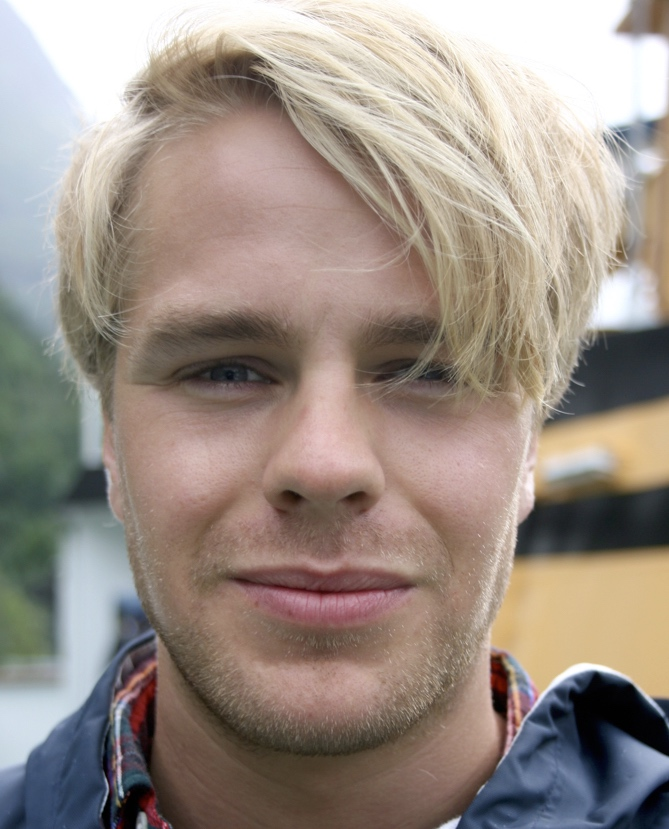
\includegraphics[width=0.15\textwidth]{pic.jpg}
\end{wrapfigure}

\MyName{Mikael Kajbring}
\MySlogan{Curriculum Vit\ae\ (\today)}

\sepspace
\sepspace

%%% Personal details
%%% ------------------------------------------------------------
\NewPart{}{}

\PersonalEntry{Address:}{{Clemensstrasse 81}, 80796 München}
\PersonalEntry{Phone:}{+ 49 (0)152/58461296}
\PersonalEntry{Mail:}{\href{mailto:appelbaum@physics.umd.edu}{kajbring@kth.se}}
\PersonalEntry{Nationality:}{Swedish}
\PersonalEntry{Born:}{03.04.1989}






%%% Work experience
%%% ------------------------------------------------------------
\NewPart{Education}{}

\EducationEntry{Master in Vehicle engineering}{2013-2018}{Royal Institute of Technology(KTH), Stockholm, Sweden}{\begin{itemize}
\item{On-going education in Mechanical engineering with focus on vehicles, transportation and production management}
\item{Basic knowledge CAD, Solid Edge}\end{itemize}}
\sepspace

\EducationEntry{Economics, law
}{2011-2012}{Uppsala University}{\begin{itemize}
\item{Basic micro- and macro-theory}
\item{Basic commercial law}\end{itemize}}

\sepspace

\EducationEntry{Upper secondary diploma, technical industrial design
}{2005-2008}{Stockholm, Sweden}{\begin{itemize}\item{Basic knowledge CAD, 3D-studiomax, AutoCAD}\end{itemize}}




%%% Work experience
%%% ------------------------------------------------------------
\NewPart{Work Experience}{(Reference on demand)}

\WorkEntry{Expoprojekt}{\href{http://expoprojekt.se}{expoprojekt.se}}{2015}{Stockholm, Sweden}{Exhibition production manager. Part-time during the whole year and different projects during summer.}

\sepspace

\WorkEntry{Jernhusen}{\href{http://jernhusen.se}{jernhusen.se}}{2014}{Stockholm, Sweden}{Organization during summer of a computer system for real estate energy. Jernhusen owns main part of the real estate connected to the Swedish railway.}

\sepspace

\WorkEntry{Alpingaraget, alpint AB}{\href{http://alpingaraget.se}{alpingaraget.se}}{2012-2015}{Stockholm, Sweden}{Part-time sales of sport goods, (mainly skis), ski service and customer service.}
\newpage

\WorkEntry{Sandgren Electronics AB}{\href{http://iphonereparation.se}{iphonereparation.se}}{2012-2013}{Gothenburg/ Stockholm, Sweden}{Summer vacation work experience and part-time. Electronic repairs, mainly cell phones.}

\sepspace

\WorkEntry{Active Ski Travel Scandinavia AB}{\href{http://www.activeski.se}{activeski.se}}{2012}{Engelberg, Switzerland}{Travel guide during winter. Responsible for guests traveling to Engelberg.}

\sepspace

\WorkEntry{Surefoot}{\href{http://www.surefoot.com}{surefoot.com}}{2011}{Verbier, Switzerland}{Part-time winter. Building custom-made ski boots. Sales of sport goods, mainly ski boots.}
\sepspace

\WorkEntry{Mässmix Design AB }{}{2009-2013}{Stockholm, Sweden}{Fulltime employee as exhibition production manager 2009. Part-time during different projects until 2013. Work-tasks: Planning, designing and manufacturing exhibitions-stands to different exhibitions through out the world.}
\sepspace

\WorkEntry{Björk and Söderqvist construction AB}{\href{http://bjorksoderqvist.com}{bjorksoderqvist.com}}{2008-2009}{Stockholm, Sweden}{Carpenter at Björk and Söderqvist during Fall 2008 and summer 2009.}

\sepspace



%%% OTHER QUALIFICATIONS
%%% ------------------------------------------------------------
\NewPart{OTHER QUALIFICATIONS}{}

\WorkEntry{Founding and developing a ski-company, Skadi skis}{\href{https://www.facebook.com/skadiskis/}{Skadiskis.se}}{2008-2013}{Stockholm, Sweden}{Production of a pair of alpine skis during the last year of upper secondary school with a friend, which later on resulted in the founding of Skadi skis.
The company produced hand-made freeride skis for the Swedish and Swiss market. All of the production was ‘in house’ and the factory location was Stockholm. Since 2013 the company is on hold due to studies. Development and testing of skis is still active.}
\sepspace

\WorkEntry{Snow safety education, 8 days}{\href{http://www.strapatser.se}{strapatser.se}}{2006}{Funäsdalen, Sweden}{Education with focus on avalanche and ski safety.}
\sepspace
\WorkEntry{Drivers license}{}{2007}{Stockholm, Sweden}{Car, quad and snowmobile}


%%% LANGUAGES
%%% ------------------------------------------------------------
\NewPart{LANGUAGES}{}

\Language{Swedish}{(mother tongue),}\Language{English}{(fluent),}\Language{German}{(B1.2),}\Language{Spanish,}{(A1)}


%%% LANGUAGES
%%% ------------------------------------------------------------
\NewPart{Interests and personality}{}

\Text{Sports and outdoor activities, mainly freeride skiing. The last couple of years I have been competing in freeride skiing and been partially living in the Swiss Alps. Through my skiing I have also developed my ski production. My friends and family form my other big interest. I see myself as a happy, outgoing and reliable person. I am a problem solver and no challenge is too big. The result of my work is often better than expected.}

\newpage


%%% Letter
%%% ------------------------------------------------------------
\NewParttwo{Anschreiben Völkl}

\sepspace



\Textlong{Praktikant im bereich entwicklung/labor ski/snowboard.}{Sehr geehrte(r) herr oder frau}{Mein Name ist Mikael Kajbring. Ich bin 26 Jahre alt und komme aus Stockholm. Ich wohne in München und bin ein Erasmus-Student an der Technischen Universität München (TUM). Ich studiere Maschinenbau/ Fahrzeugtechnik im dritten Jahr mit Ausrichtung Management. Nach dem Abitur an einer technischen Schule habe ich eine Ski-Firma (Skadi-skis) gegründet, in der ich Freerideski für den schwedischen und schweizer Markt angefertigt habe. Die Firma gibt es jetzt nicht mehr, aber ich entwickle weiter Ski für mich und Freunde. Ich habe mit vielen Materialien gearbeitet wie Titanal, Polyurethan, Kohlefaser und Bambus. Weil die Firma nicht groß war, habe ich Produktion, Marketing und Vertrieb geleitet. Ich habe auch Fertigkeiten mit CAD- und Graphikdesign-Programmen, weil ich alle Entwürfe und Topsheets selbst gemacht habe. Während meines Studiums habe ich auch in einem kleinen Skigeschäft in Stockholm gearbeitet. 
Meine Leidenschaften sind Skifahren und das Leben in der Natur. Zwischen 2010 und 2014 habe ich an Wettkämpfen der Freeride World Qualifier teilgenommen und ich habe viele Freunde in der Freeride World Tour, unter anderem euren Fahrer Sam Smoothy. 
Ich sehe mich selbst als einen glücklichen und sympathischen Menschen. Meine englischen Sprachkenntnisse sind sehr gut und durch das Erlernen der deutschen Sprache hoffe ich meine sozialen Fähigkeiten zu erweitern. Nach dem Studium will ich in der Entwicklung von Sportgeräten arbeiten und ich hoffe, ich kann bei Völkl damit anfangen.
Mit diesem Hintergrund möchte ich fragen, ob Sie für mich eine Praktikumstelle im nächsten Jahr haben.}{Mit freundlichen Grüßen, Mikael Kajbring}

\sepspace

\begin{wrapfigure}{l}{\textwidth}
		\vspace{5em}
        \centering
		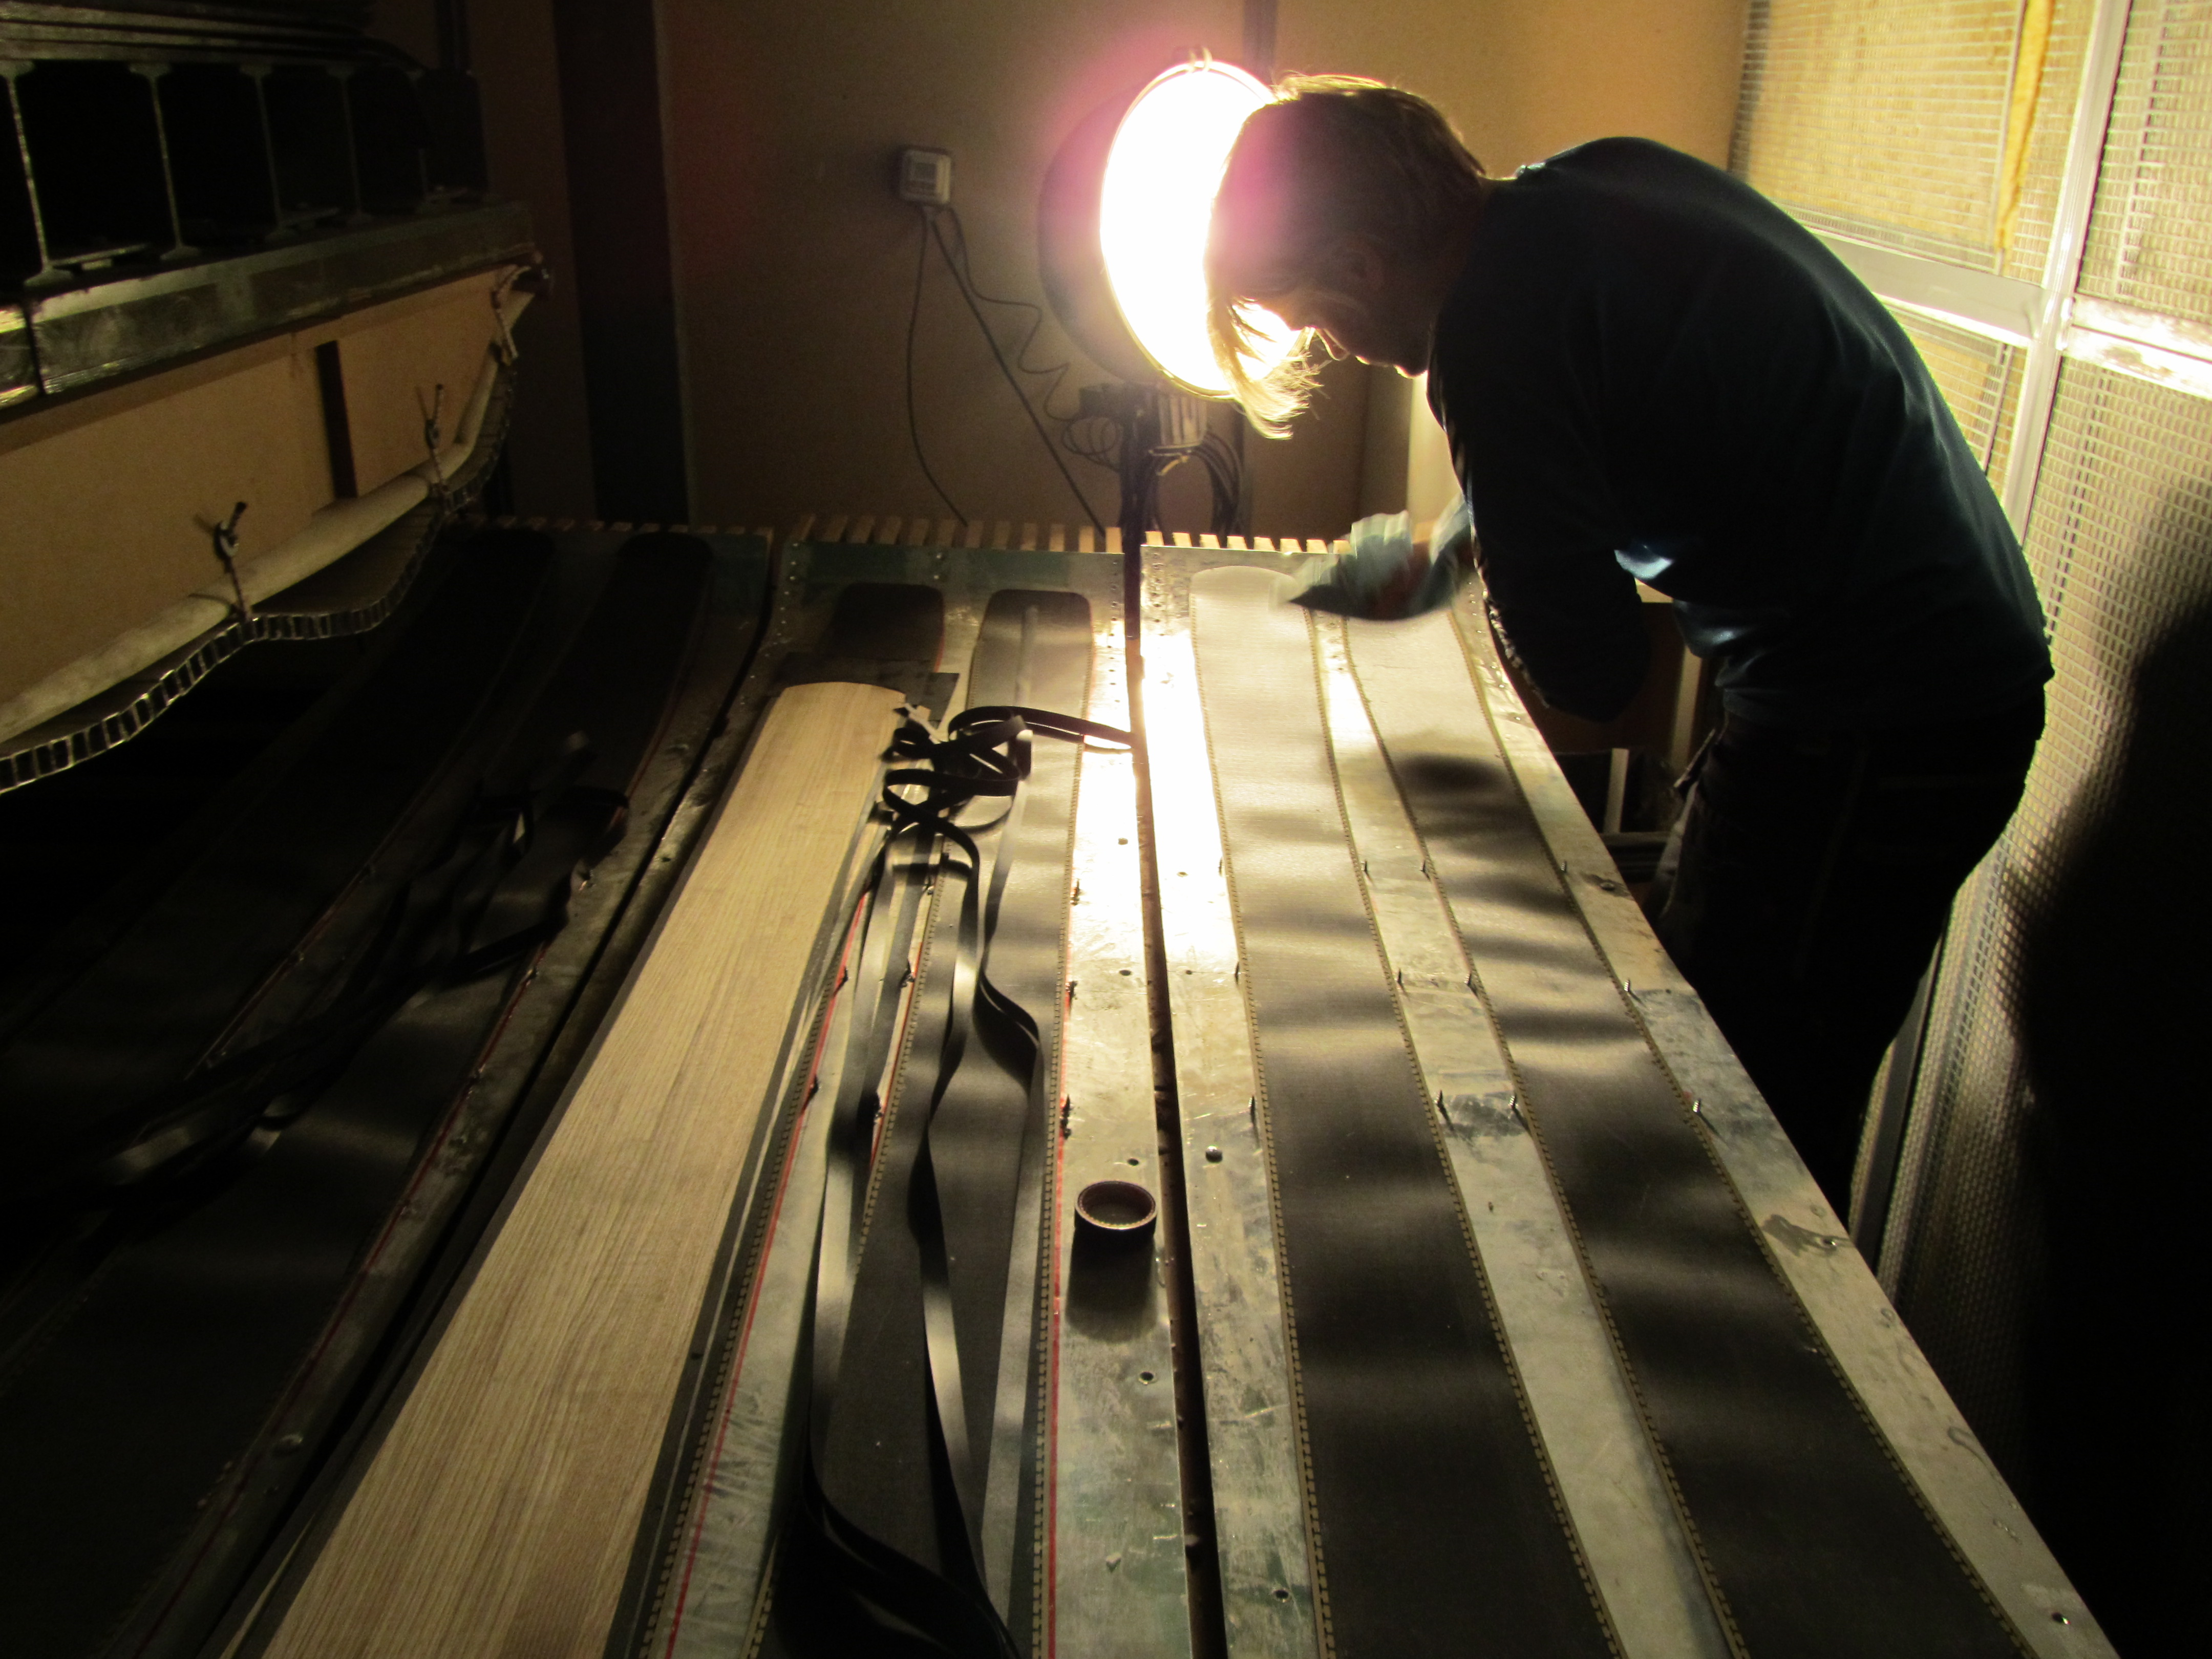
\includegraphics[height=0.25\textwidth]{IMG_0068.JPG}
        \hspace{1em}
        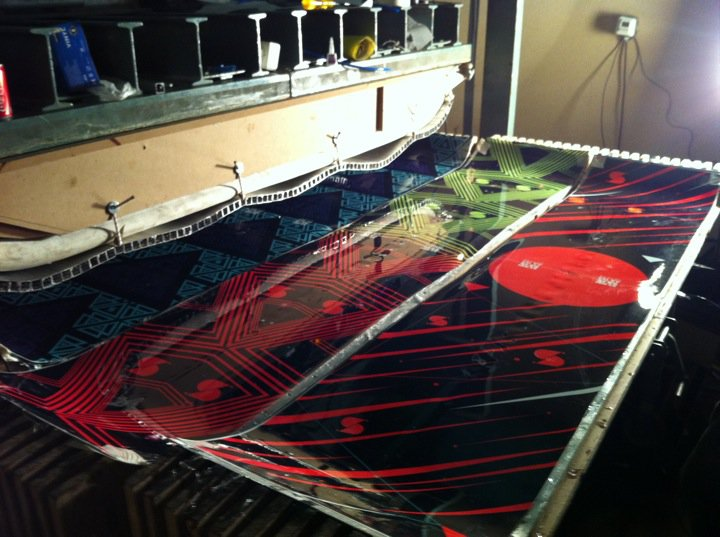
\includegraphics[height=0.25\textwidth]{154327_165817636790533_1488132_n.jpg}
        
\end{wrapfigure}

\begin{wrapfigure}{l}{\textwidth}
		\vspace{1em}
        \centering            
        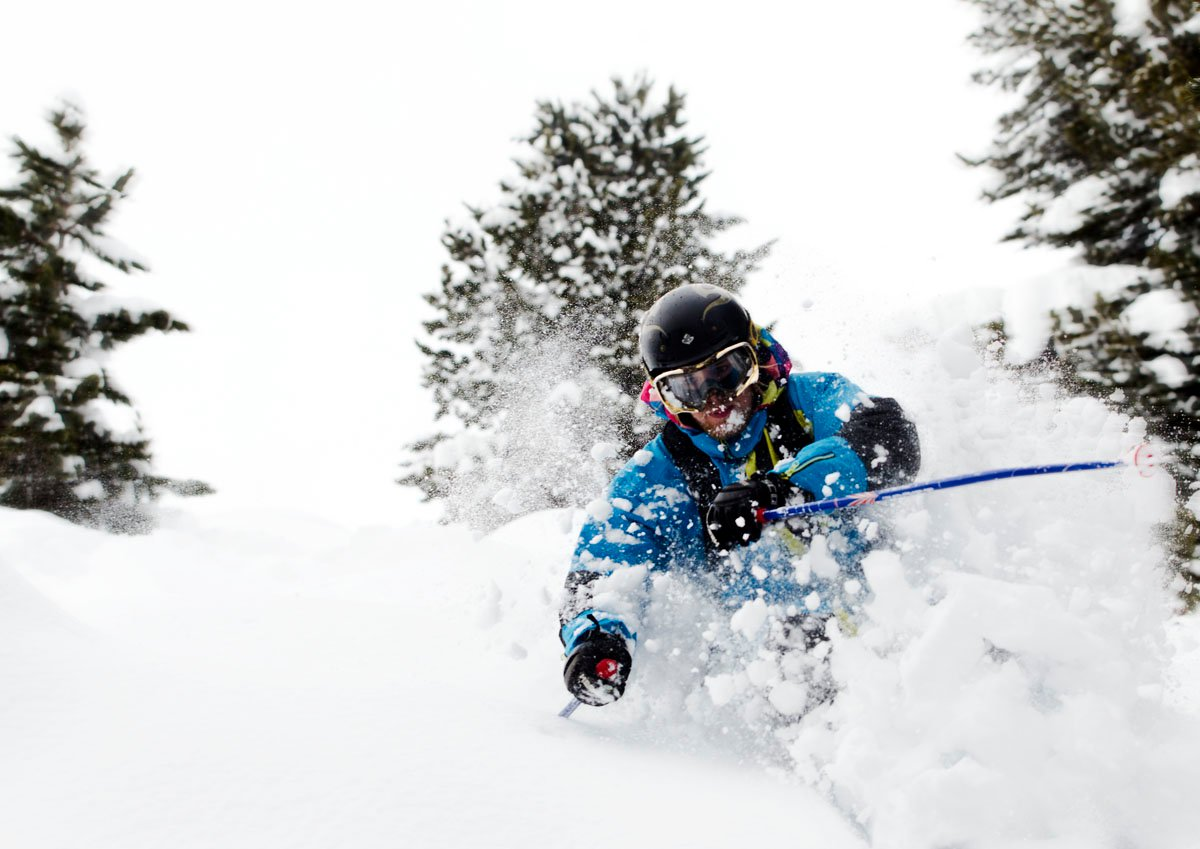
\includegraphics[height=0.25\textwidth]{133107_166579826714314_3462381_o.jpg}
        
\end{wrapfigure}


\end{document}
